% Eigenspaces of A = [1 6; 5 2] (Lay 2015, Sec. 5.1): two lines through the origin.
% lambda = 7: span{(1,1)}; lambda = -4: span{(-6,5)}. A non-eigenvector w = (-1/2,-1)
% is shown for contrast: A w = (-13/2,-9/2) leaves w's line.
\begin{center}
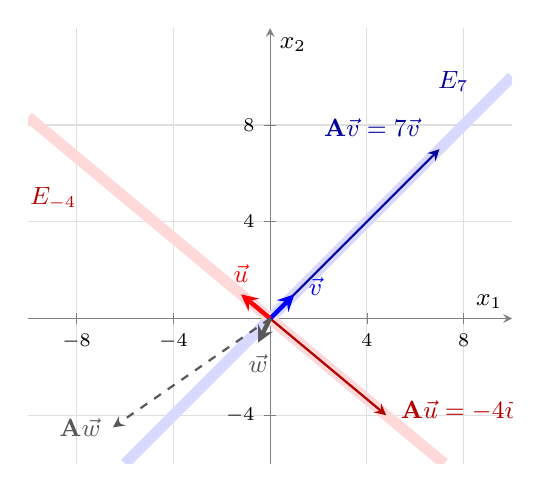
\begin{tikzpicture}
\begin{axis}[
  width=0.68\linewidth,
  axis equal image,
  axis lines=center,
  axis line style={gray},
  xlabel={$x_1$}, ylabel={$x_2$},
  label style={font=\small},
  xmin=-10, xmax=10, ymin=-6, ymax=12,
  xtick={-8,-4,4,8}, ytick={-4,4,8},
  tick label style={font=\scriptsize},
  grid=major, grid style={gray!25},
]
% eigenspace lambda = 7: x2 = x1 (wide pale band so the arrows on it stay visible)
\addplot[domain=-6:10, line width=4pt, blue!15, samples=2] {x};
\node[blue!60!black, font=\small, anchor=south east] at (axis cs:8.6,9) {$E_{7}$};
% eigenspace lambda = -4: 5 x1 + 6 x2 = 0
\addplot[domain=-10:7.2, line width=4pt, red!15, samples=2] {-5*x/6};
\node[red!70!black, font=\small, anchor=north east] at (axis cs:-7.6,5.8) {$E_{-4}$};
% A v = 7 v for v = (1,1)
\draw[thick, blue!60!black, -stealth] (axis cs:0,0) -- (axis cs:7,7);
\node[blue!60!black, font=\small, anchor=south east] at (axis cs:6.6,7.1) {$\mathbf{A}\vec{v} = 7\vec{v}$};
% A u = -4 u for u = (-1.2, 1): flipped and stretched
\draw[thick, red!70!black, -stealth] (axis cs:0,0) -- (axis cs:4.8,-4);
\node[red!70!black, font=\small, anchor=west] at (axis cs:5,-3.8) {$\mathbf{A}\vec{u} = -4\vec{u}$};
% the eigenvectors themselves, on top
\draw[ultra thick, blue, -stealth] (axis cs:0,0) -- (axis cs:1,1);
\node[blue, font=\small, anchor=west] at (axis cs:1.2,1.3) {$\vec{v}$};
\draw[ultra thick, red, -stealth] (axis cs:0,0) -- (axis cs:-1.2,1);
\node[red, font=\small, anchor=south] at (axis cs:-1.2,1.1) {$\vec{u}$};
% non-eigenvector w = (-1/2,-1), A w = (-13/2,-9/2)
\draw[ultra thick, gray!70!black, -stealth] (axis cs:0,0) -- (axis cs:-0.5,-1);
\node[gray!70!black, font=\small, anchor=north] at (axis cs:-0.5,-1.1) {$\vec{w}$};
\draw[thick, gray!70!black, -stealth, dashed] (axis cs:0,0) -- (axis cs:-6.5,-4.5);
\node[gray!70!black, font=\small, anchor=east] at (axis cs:-6.6,-4.5) {$\mathbf{A}\vec{w}$};
\end{axis}
\end{tikzpicture}
\end{center}
